\documentclass[../Draft_harmonization_paper.tex]{subfiles}
% \documentclass{article}
% \usepackage[utf8]{inputenc}
% \usepackage{hyperref}
% \usepackage{float}
% \usepackage[table,xcdraw]{xcolor}
% \usepackage{color, colortbl}
% \usepackage{longtable}
% %\usepackage[sort&compress,square,comma,authoryear]{natbib}
% \usepackage{booktabs}
% \usepackage{graphicx}
% \graphicspath{{/home/kunz/Dokumente/Projects/Trait_DB/Invertebrate_traits/Paper/Figures/}}
% \usepackage{longtable}
% \usepackage{rotating}
% \usepackage{geometry}
% \usepackage{array}

% \definecolor{Gray}{gray}{0.9}

% \newcommand{\specialcell}[2][c]{%
%   \begin{tabular}[#1]{@{}c@{}}#2\end{tabular}}

\begin{document}
%! Trait (species) scores along segments of river

\subsection*{Re-analysis of Szöcs et al. using harmonized and aggregated grouping features}

The original RDA in Szöcs et al. (\cite{szocs_effects_2014}) indicated that downstream sites (high salinity) were characterized by the traits feeding mode shredder, ovoviviparity, multivoltinism, long life cycle ($> 1$ year), and gill respiration and upstream sites (low salinity) were characterized by univoltinism, oviposition in clutches and short life cycle duration ($< 1$ year). Using harmonized grouping features led to slightly different results in comparison to the original analysis (Figure \ref{fig:rda_species_scores} and SI). According to the RDA of the trait composition, downstream sites were characterized by taxa that possess the traits multivoltinism and ovoviviparity and upstream sites were characterized by univoltine taxa that lay their eggs in an aquatic environment. The traits shredder, gill respiration and long life cycle duration did not anymore characterize sites with high salinisation. Also, the trait short life cycle duration year did not characterise sites upstream sites with low salinity.% TODO: two graphics in one in the results part
We also constructed the linear models of the original analyses, using the traits on bith extremes of the conductivity axis and found results similar to the original analyses (Table S\ref{stab:linear_models_new} and S\ref{stab:linear_models_edi}).

Results changed slightly when comparing at family-level aggregated traits to the original analysis. (Figure \ref{fig:rda_species_scores}). 
% Weighted, direct_agg (mean) and direct_agg (median) similar
% In addition to the results of harmonized: + gil respiration, long life cycle duration
% Short life cycle duration for upstream sites

% Stepwise_agg (mean), stepwise_agg (median) similar 
% In addition to the results of harmonized: + resp_gil

% In our comparison the family-level aggregation yielded to the least change in species scores of all methods.

\begin{figure}[H]
    \label{fig:rda_species_scores}
    \centering
    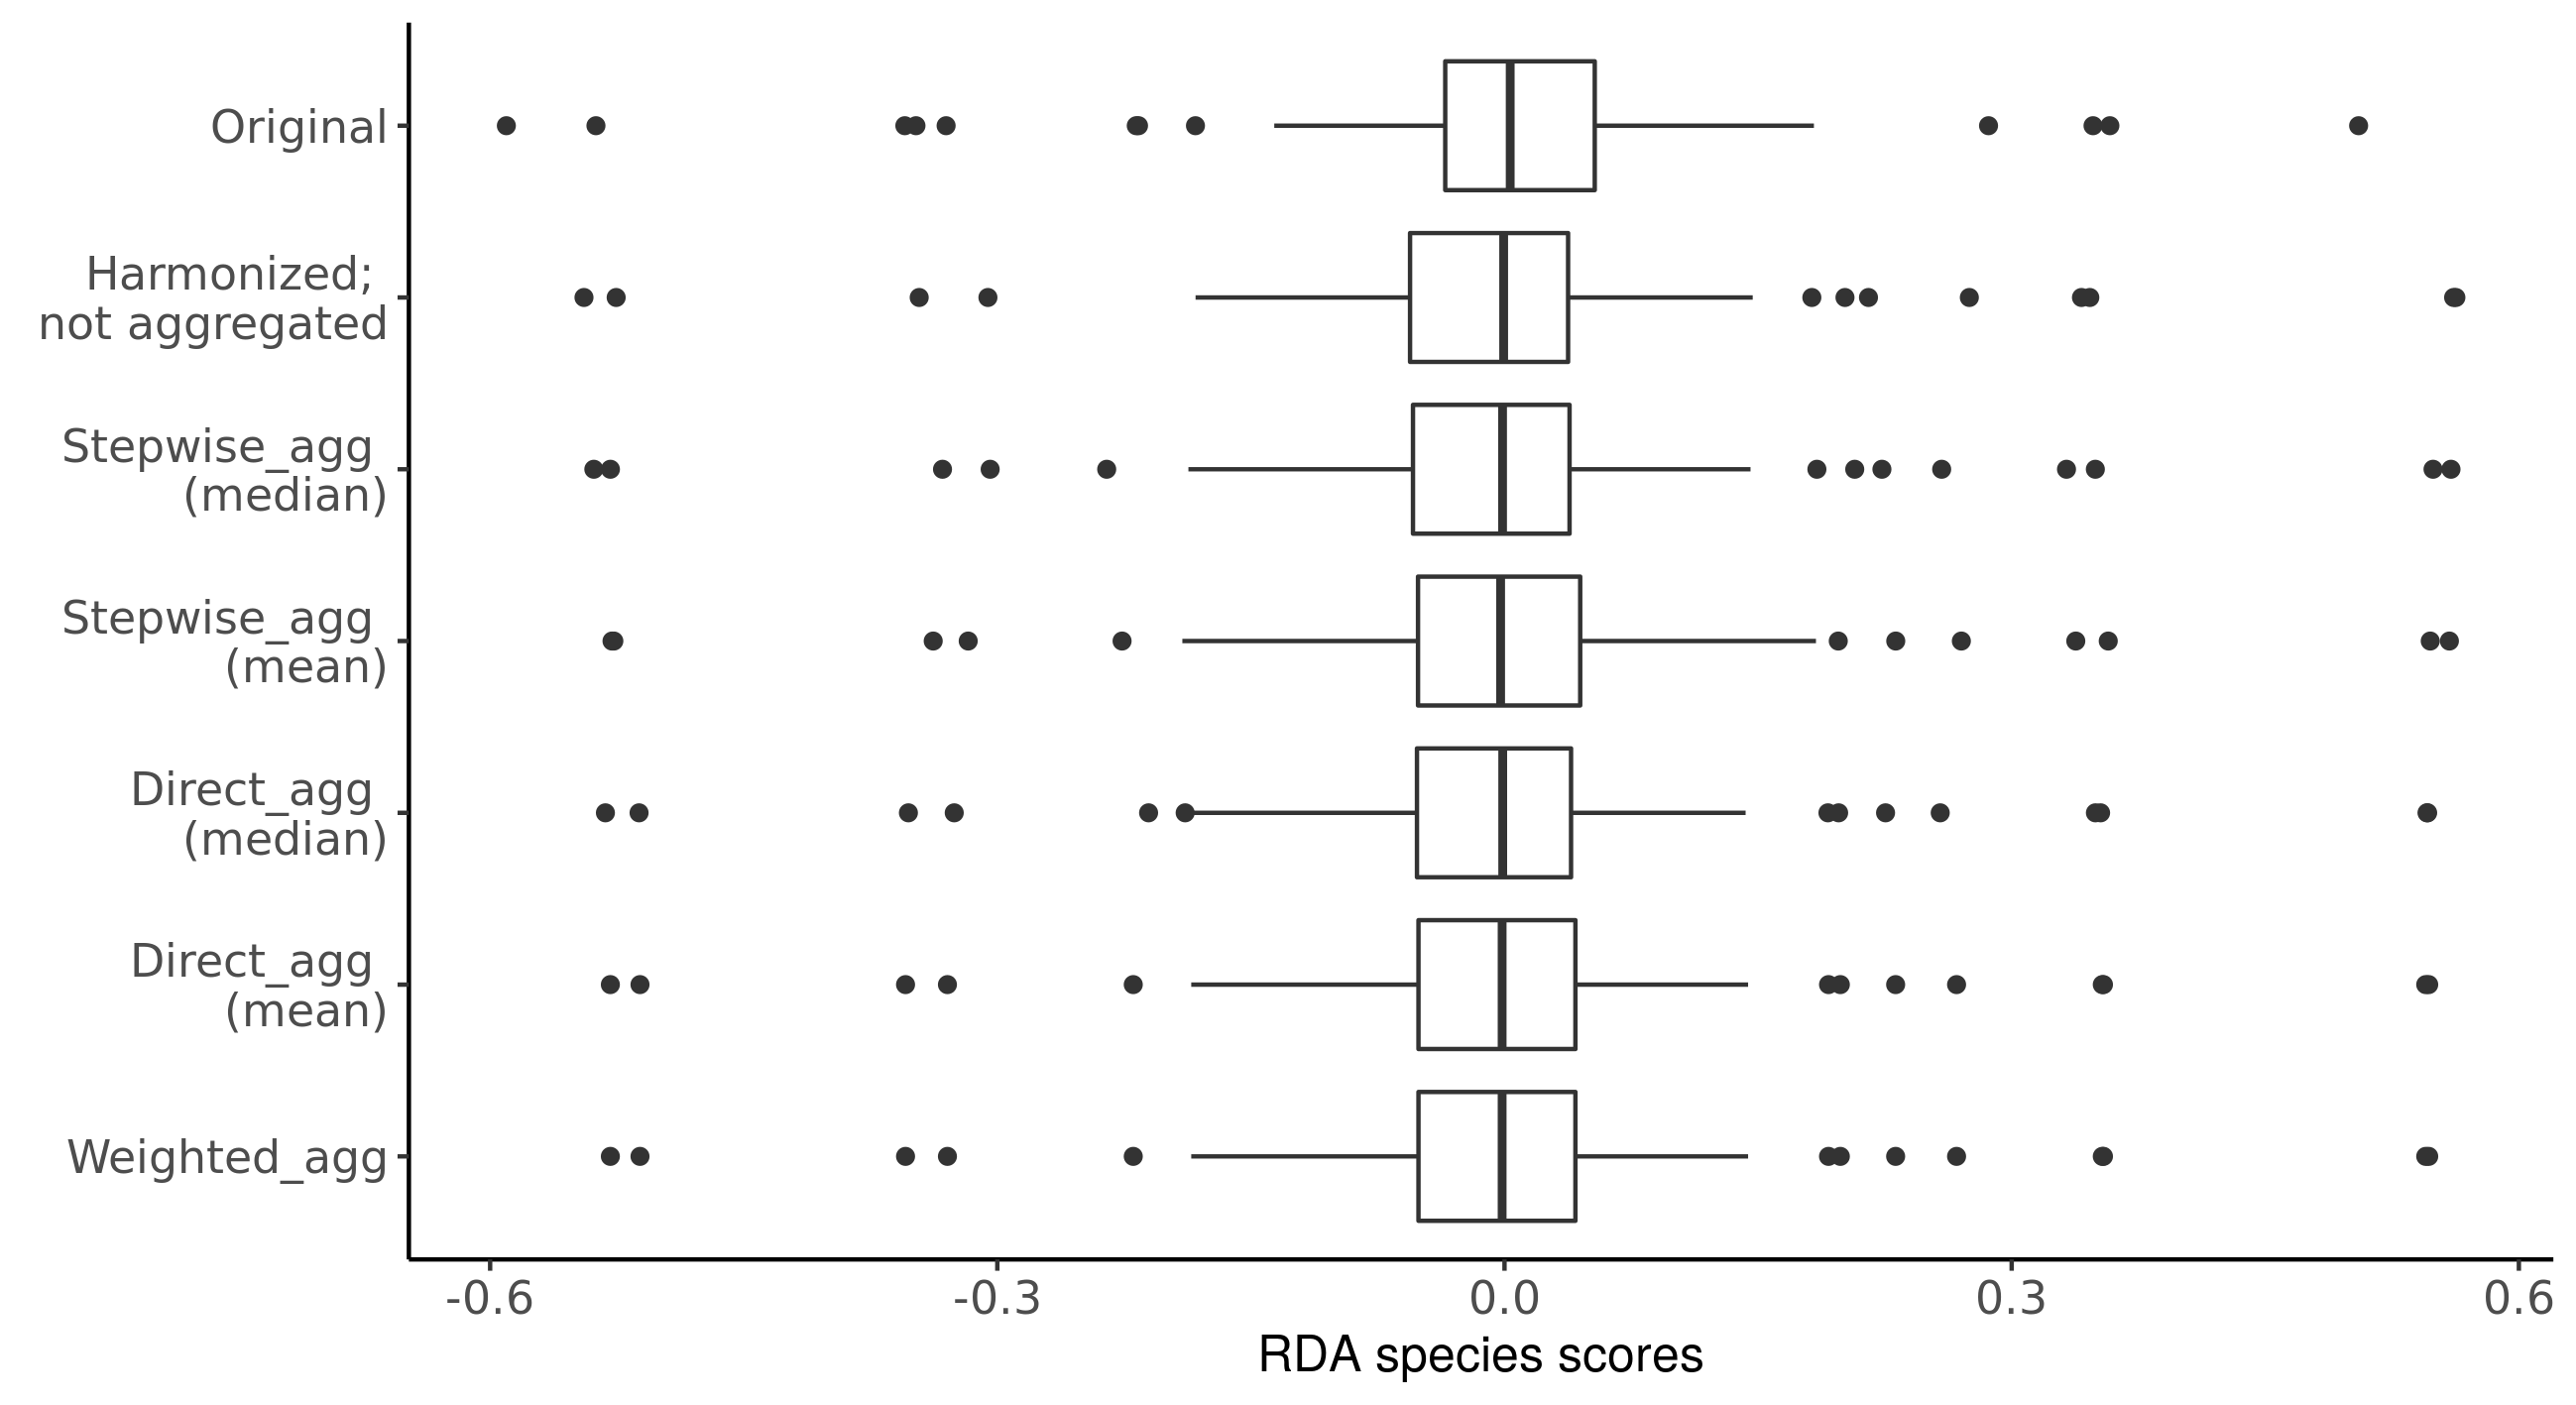
\includegraphics[width=16.5cm, height=10cm]{Species_scores_rda.png}
    \caption{Species scores obtained by RDA from the original analysis \cite{szocs_effects_2014}, using harmonized grouping features, and using harmonized grouping features with trait affinities aggregated to family-level.}
    \label{fig:rda_species_scores}
\end{figure}

\end{document}